% chuong5.tex — sửa nội dung chương ở đây
\section{Giải pháp và hiện thực}\label{sec:5}

\subsection{Đề xuất giải pháp}\label{sec:5.1}

Mỗi giải pháp gắn với một hoặc vài thách thức ở chương 4, theo bảng sau. Các quy trình dưới đây là đề xuất của nhóm, chưa phải kết quả triển khai thực tế. Giải pháp 1 được hiện thực bằng công cụ demo, giải pháp 4 và 6 bằng tài liệu PoC ở mục~\ref{sec:5.2}; giải pháp 2, 3 và 5 dừng ở mức đề xuất.

{\small\setstretch{1.1}
\begin{table}[H]
\centering
\caption{Các giải pháp và thách thức tương ứng}\label{tab:5.6}
\begin{tabularx}{\textwidth}{>{\raggedright\arraybackslash}l>{\hsize=1.062\hsize\raggedright\arraybackslash}X>{\hsize=1.286\hsize\raggedright\arraybackslash}X>{\hsize=0.652\hsize\raggedright\arraybackslash}X}
\toprule
\textbf{Giải pháp} & \textbf{Nội dung} & \textbf{Thách thức xử lý} & \textbf{Mức hiện thực} \\
\midrule
Giải pháp 1 & Phát hiện tin có dấu hiệu vi phạm & Khối lượng tin đăng; tin ngụy trang & Demo (\ref{sec:5.2.1}) \\
Giải pháp 2 & Bảo vệ tài khoản trên nền tảng gốc & Tài khoản đổi chủ & Đề xuất \\
Giải pháp 3 & Truy nguồn rò rỉ dữ liệu & Dữ liệu dễ sao chép & Đề xuất \\
Giải pháp 4 & Kiểm soát người bán & Vỏ bọc doanh nghiệp & PoC tài liệu (\ref{sec:5.2.2}) \\
Giải pháp 5 & Ma trận trách nhiệm pháp lý & Văn bản thay đổi theo thời gian; ranh giới trách nhiệm & Đề xuất \\
Giải pháp 6 & Phối hợp xử lý & Hạ tầng ở nước ngoài; dữ liệu nằm ở nhiều bên & PoC tài liệu (\ref{sec:5.2.2}) \\
\bottomrule
\end{tabularx}
\end{table}}

\subsubsection{Giải pháp 1: Phát hiện tin có dấu hiệu vi phạm}\label{sec:5.1.1}

\begin{itemize}
\item \textbf{Mục tiêu:} giảm khối lượng đọc thủ công và ưu tiên những tin cần kiểm tra.
\item \textbf{Căn cứ:} quy định về bảo vệ dữ liệu cá nhân và trách nhiệm kiểm soát nội dung của nền tảng~\cite{luat-bvdlcn-2025,vbhn-tmdt-2020,cuc-tmdt-2026}; quy định về hệ thống trí tuệ nhân tạo~\cite{luat-ai-2025}.
\item \textbf{Cách làm:} chuẩn hóa nội dung tin đăng, quét bằng từ khóa và biểu thức chính quy kết hợp với mô hình học máy, rồi đưa ra cảnh báo có lý do để người kiểm tra xem lại.
\item \textbf{Đầu ra:} danh sách cảnh báo và nhật ký bằng chứng. Công cụ không tự kết luận ai vi phạm. Demo dùng dữ liệu do nhóm tự tạo, không thu thập dữ liệu rò rỉ thật.
\end{itemize}
\subsubsection{Giải pháp 2: Bảo vệ tài khoản trên nền tảng gốc}\label{sec:5.1.2}

\begin{itemize}
\item \textbf{Mục tiêu:} phát hiện tài khoản bị bán hoặc chuyển cho người khác dùng.
\item \textbf{Cách làm:} nền tảng gốc (mạng xã hội, dịch vụ thư điện tử) kết hợp các tín hiệu như thời điểm tạo tài khoản, việc đổi thiết bị và số lần yêu cầu xác thực. Khi thấy bất thường, nền tảng cảnh báo, yêu cầu xác thực bổ sung và hỗ trợ chủ tài khoản khiếu nại. Việc theo dõi chỉ ghi nhận sự kiện yêu cầu và xác minh, không lưu giá trị mã OTP hay mật khẩu.
\item \textbf{Căn cứ:} trách nhiệm bảo vệ dữ liệu và bảo đảm an ninh hệ thống~\cite{luat-bvdlcn-2025,luat-anm-2025}.
\item \textbf{Đầu ra:} hồ sơ cảnh báo tài khoản. Giải pháp ở mức đề xuất.
\end{itemize}
\subsubsection{Giải pháp 3: Truy nguồn rò rỉ dữ liệu}\label{sec:5.1.3}

\begin{itemize}
\item \textbf{Mục tiêu:} khi dữ liệu bị rao bán, xác định được dữ liệu rò rỉ từ đâu và hạn chế thiệt hại.
\item \textbf{Cách làm:} bên kiểm soát dữ liệu quản lý quyền truy cập và lưu nhật ký mỗi lần xuất hoặc chia sẻ dữ liệu. Khi có sự cố, bên kiểm soát bảo toàn chứng cứ, khoanh vùng, truy vết và thông báo vi phạm theo Điều 23 Luật Bảo vệ dữ liệu cá nhân 2025. Mốc thông báo trong 72 giờ chỉ áp dụng cho đúng chủ thể và trường hợp mà Điều 23 quy định~\cite{luat-bvdlcn-2025,nd356-2025}.
\item \textbf{Đầu ra:} hồ sơ ứng phó sự cố. Truy vết không bảo đảm tìm được nguồn hay xóa được mọi bản sao. Giải pháp ở mức đề xuất.
\end{itemize}
\subsubsection{Giải pháp 4: Kiểm soát người bán}\label{sec:5.1.4}

\begin{itemize}
\item \textbf{Mục tiêu:} ngăn hàng hóa bị cấm xuất hiện trên sàn ngay từ khâu mở gian hàng.
\item \textbf{Cách làm:} xác minh người bán, kiểm tra hàng hóa và dịch vụ đăng bán, đối soát thanh toán qua đơn vị được cấp phép, và xử lý vi phạm có căn cứ. Xác minh danh tính không làm hàng hóa bị cấm trở nên hợp pháp, nên bước kiểm tra hàng hóa vẫn bắt buộc.
\item \textbf{Căn cứ:} quy định về bảo vệ dữ liệu, thương mại điện tử và thanh toán~\cite{luat-bvdlcn-2025,nd356-2025,vbhn-tmdt-2020,nd52-2024,luat-tmdt-2025}. Theo Cục Thương mại điện tử, nghĩa vụ xác thực điện tử danh tính người bán áp dụng từ 1/1/2027 và không hồi tố cho hoạt động trước đó~\cite{cuc-tmdt-2026}.
\item \textbf{Đầu ra:} các chính sách Đăng ký, Hàng cấm, Gỡ tin, Giáo dục, luồng A (nền tảng tự kiểm soát) và bộ tiêu chí nhận diện “chợ dữ liệu”, hiện thực ở dạng PoC tài liệu theo cách tiếp cận 3P tại~\ref{sec:5.2.2}.
\end{itemize}
\subsubsection{Giải pháp 5: Ma trận trách nhiệm pháp lý}\label{sec:5.1.5}

\begin{itemize}
\item \textbf{Mục tiêu:} giúp cơ quan và nền tảng xác định đúng chủ thể, đúng văn bản cho từng hành vi.
\item \textbf{Cách làm:} lập ma trận gồm hành vi, chủ thể, thời điểm, nghĩa vụ và chứng cứ cần có; quy định rõ người kiểm tra và người phê duyệt. Cảnh báo tự động không tự tạo ra quyền phong tỏa tiền; mọi biện pháp như vậy phải có căn cứ pháp lý riêng.
\item \textbf{Căn cứ:} các văn bản ở mục~\ref{sec:2.2} và khung pháp luật hiện hành~\cite{luat-bvdlcn-2025,nd356-2025,luat-anm-2025,luat-tmdt-2025}.
\item \textbf{Đầu ra:} ma trận nghĩa vụ. Giải pháp ở mức đề xuất, chưa kiểm chứng hiệu quả thực thi.
\end{itemize}
\subsubsection{Giải pháp 6: Phối hợp xử lý}\label{sec:5.1.6}

\begin{itemize}
\item \textbf{Mục tiêu:} biến một tín hiệu nghi vấn thành hồ sơ có đầu mối theo dõi.
\item \textbf{Cách làm:} tiếp nhận, sàng lọc, bảo toàn chứng cứ, chuyển đúng thẩm quyền, rồi nhận phản hồi và theo dõi. Yêu cầu nhà cung cấp hạ tầng xử lý (ví dụ tạm ngừng tên miền hay máy chủ) phải có căn cứ hợp pháp.
\item \textbf{Căn cứ:} quy định về an ninh mạng, bảo vệ dữ liệu và nghĩa vụ phối hợp~\cite{luat-bvdlcn-2025,nd356-2025,luat-anm-2025,cuc-tmdt-2026,nd327-2026,nd333-2026}.
\item \textbf{Đầu ra:} các chính sách Lưu trữ, Phối hợp, luồng B (nền tảng phối hợp với cơ quan), quy trình phía cơ quan chức năng, bảng thủ tục có thời hạn theo luật và biểu mẫu tiếp nhận tố giác, hiện thực ở dạng PoC tài liệu theo cách tiếp cận 3P tại~\ref{sec:5.2.2}.
\end{itemize}
\subsection{Hiện thực giải pháp}\label{sec:5.2}

Mục này hiện thực ba giải pháp: giải pháp 1 bằng một công cụ demo (\ref{sec:5.2.1}), giải pháp 4 và 6 bằng tài liệu PoC theo cách tiếp cận 3P gồm chính sách, quy trình và thủ tục (\ref{sec:5.2.2}). Giải pháp 2, 3 và 5 dừng ở mức đề xuất như đã trình bày ở~\ref{sec:5.1}.

\subsubsection{Demo kỹ thuật giải pháp 1: Công cụ phát hiện tin đăng vi phạm}\label{sec:5.2.1}

Mã nguồn: notebook Colab \texttt{Demo\_\allowbreak{}phat\_\allowbreak{}hien\_\allowbreak{}tin\_\allowbreak{}dang.ipynb}, chạy bằng Runtime → Run all trong khoảng 1–2 phút.

\paragraph{Giới thiệu}

Công cụ đọc nội dung một tin đăng và cho biết tin đó có dấu hiệu thuộc một trong ba nhóm hành vi đã phân tích ở chương 3 hay không: mua bán dữ liệu cá nhân, mua bán tài khoản mạng xã hội và thư điện tử, cung cấp dịch vụ xác thực tài khoản hộ. Mục tiêu là giải quyết hai thách thức ở mục~\ref{sec:4.1}: khối lượng tin đăng quá lớn để đọc thủ công, và tin viết lách, ngụy trang.

\begin{itemize}
\item \textbf{Input:} nội dung chữ của một tin đăng.
\item \textbf{Output:} một trong ba quyết định (CHẶN, CHUYỂN NGƯỜI DUYỆT, CHO PHÉP), kèm loại vi phạm nghi ngờ, điểm rủi ro từ 0 đến 1 và danh sách lý do.
\end{itemize}
Toàn bộ dữ liệu trong demo do nhóm tự tạo; số điện thoại, CCCD, email đều là số bịa. Nhóm không thu thập dữ liệu từ trang taphoammo hay bản lưu trữ của trang. Công cụ chỉ gắn cờ tin nghi vấn để người kiểm tra xem lại, không tự kết luận ai vi phạm.

\begin{figure}[H]
\centering
% Luồng xử lý của công cụ GP1
\setstretch{1}
\begin{tikzpicture}[font=\footnotesize,
  box/.style={draw, rounded corners=2pt, align=center, minimum height=1.1cm, text width=2.3cm, fill=#1},
  box/.default=white, arr/.style={-{Stealth[length=2mm]}, thick}]
  \node[box=gray!12]   (in)   at (0,0)     {Tin đăng\\(nội dung chữ)};
  \node[box=gray!12]   (norm) at (3.1,0)   {Chuẩn hóa chữ,\\chống ngụy trang};
  \node[box=blue!10]   (kw)   at (6.2,0.9) {Quét từ khóa\\+ Regex};
  \node[box=green!12]  (ml)   at (6.2,-0.9){Học máy\\TF-IDF + LR};
  \node[box=orange!15] (mix)  at (9.3,0)   {Kết hợp,\\tính điểm rủi ro};
  \node[box=red!10, text width=3.3cm]  (dec) at (9.3,-2.6) {CHẶN / CHUYỂN NGƯỜI DUYỆT / CHO PHÉP, kèm lý do};
  \node[box=gray!12, text width=3.3cm] (log) at (4.6,-2.6) {Nhật ký bằng chứng\\(che dữ liệu, SHA-256)};
  \draw[arr] (in) -- (norm);
  \draw[arr] (norm.east) -- ++(0.25,0) |- (kw.west);
  \draw[arr] (norm.east) -- ++(0.25,0) |- (ml.west);
  \draw[arr] (kw.east) -- ++(0.25,0) |- (mix.west);
  \draw[arr] (ml.east) -- ++(0.25,0) |- (mix.west);
  \draw[arr] (mix) -- (dec);
  \draw[arr] (dec) -- (log);
\end{tikzpicture}

\caption{Luồng xử lý của công cụ phát hiện tin đăng vi phạm}
\label{fig:5.1}
\end{figure}

\paragraph{Chuẩn bị dữ liệu huấn luyện}

Module học máy cần học từ các tin đã gán nhãn. Nhóm viết 52 mẫu câu có chỗ trống cho bốn nhãn (BAN\_\allowbreak{}DLCN, BAN\_\allowbreak{}TAI\_\allowbreak{}KHOAN, DICH\_\allowbreak{}VU\_\allowbreak{}XAC\_\allowbreak{}THUC, HOP\_\allowbreak{}LE), rồi điền ngẫu nhiên nền tảng, giá, số lượng, số điện thoại giả vào chỗ trống. Kết quả là 1.024 tin huấn luyện. Nhãn hợp lệ có cả tin dễ nhầm, chẳng hạn khóa học bảo mật hay tư vấn tuân thủ pháp luật dữ liệu, vì những tin này cũng chứa chữ “dữ liệu”, “tài khoản”, “OTP”.

Ví dụ, mẫu câu “Thuê số nhận OTP \{nen\_\allowbreak{}tang\} giá \{gia\}/lần, có API tự động” sinh ra các tin như “Thuê số nhận OTP Zalo giá 15k/lần, có API tự động”.

\paragraph{Hai module phát hiện}

\textbf{Module 1: Quét từ khóa + Regex.} Bước đầu chuẩn hóa chữ để chống ngụy trang: bỏ dấu, đổi số giống chữ về chữ, ghép chữ bị tách (“d.a.t.a” thành “data”, “0tp” thành “otp”). Sau đó module dùng biểu thức chính quy (regex) tìm số CCCD, số điện thoại, email dán trong tin, cộng điểm theo bộ từ khóa có trọng số của từng loại vi phạm, và trừ điểm khi gặp ngữ cảnh hợp lệ (“chính hãng”, “hóa đơn”, “khóa học”). Một số điện thoại đơn lẻ được coi là số liên hệ; tin chỉ bị coi là có mẫu dữ liệu cá nhân khi có số CCCD hoặc từ hai giá trị trở lên.

\begin{lstlisting}[language=Python, caption={Biểu thức chính quy và bộ từ khóa (trích)}]
RE_SDT  = re.compile(r"(?<!\d)(?:\+84|0)[35789](?:[\s\.\-]?\d){8}(?!\d)")   # SDT di dong
RE_CCCD = re.compile(r"(?<!\d)0\d{11}(?!\d)")                                # CCCD 12 so
TU_KHOA["DICH_VU_XAC_THUC"] = {"otp": 2.0, "thue so": 2.0, "sim nhan": 2.0, "xac thuc ho": 3.0, ...}
\end{lstlisting}

\textbf{Module 2: Học máy (TF-IDF + Logistic Regression).} TF-IDF biến mỗi tin thành một vector số, dựa trên tần suất của từ, cụm hai từ và cụm 2–5 ký tự; cụm ký tự giúp mô hình chịu được lỗi chính tả và cách viết dính. Logistic Regression học từ 1.024 tin huấn luyện để ước lượng xác suất tin thuộc mỗi nhãn; xác suất vi phạm bằng 1 trừ xác suất hợp lệ.

\begin{lstlisting}[language=Python, caption={Mô hình TF-IDF kết hợp Logistic Regression}]
mo_hinh = Pipeline([
    ("dac_trung", FeatureUnion([
        ("tu",    TfidfVectorizer(preprocessor=chuan_hoa, ngram_range=(1, 2))),
        ("ky_tu", TfidfVectorizer(preprocessor=chuan_hoa, analyzer="char_wb", ngram_range=(2, 5))),
    ])),
    ("phan_loai", LogisticRegression(C=5.0, class_weight="balanced")),
])
mo_hinh.fit(du_lieu_huan_luyen["noi_dung"], du_lieu_huan_luyen["nhan"])
\end{lstlisting}

Sau khi huấn luyện, các từ mô hình coi là đặc trưng nhất gồm “data”, “sđt”, “họ tên” cho nhóm mua bán dữ liệu cá nhân; “acc”, “reg”, “mail” cho nhóm mua bán tài khoản; “thuê số”, “xác minh” cho nhóm dịch vụ xác thực hộ.

\textbf{Kết hợp hai module.} Điểm rủi ro = 0,6 × xác suất vi phạm của học máy + 0,4 × điểm quét từ khóa. Quyết định theo bảng sau:

{\small\setstretch{1.1}
\begin{table}[H]
\centering
\caption{Quy tắc ra quyết định của công cụ}\label{tab:5.7}
\begin{tabularx}{\textwidth}{>{\hsize=1.506\hsize\raggedright\arraybackslash}X>{\hsize=0.494\hsize\raggedright\arraybackslash}X}
\toprule
\textbf{Điều kiện} & \textbf{Quyết định} \\
\midrule
Có mẫu dữ liệu cá nhân (CCCD, hoặc từ 2 số điện thoại/email) kèm từ khóa vi phạm; hoặc điểm rủi ro ≥ 0,70 và module quét từ khóa có tìm thấy dấu hiệu & CHẶN \\
Điểm rủi ro ≥ 0,40, hoặc riêng một module ≥ 0,40, nhưng chưa đủ điều kiện chặn & CHUYỂN NGƯỜI DUYỆT \\
Các trường hợp còn lại & CHO PHÉP \\
\bottomrule
\end{tabularx}
\end{table}}

Muốn chặn thẳng thì phải có dấu hiệu cụ thể để ghi vào lý do, nên chỉ riêng học máy nghi ngờ thì chưa đủ. Chuyển người duyệt là bước an toàn, nên chỉ cần một module nghi ngờ. Khi triển khai thực tế, CHẶN chỉ có nghĩa là tạm ẩn tin và chuyển người duyệt xác nhận; công cụ không tự gỡ tin hay khóa tài khoản (xem phần tuân thủ cuối mục này).

\paragraph{Dữ liệu kiểm tra}

Bộ kiểm tra gồm 120 tin viết riêng, không trùng tin nào với dữ liệu huấn luyện: 60 tin vi phạm (20 tin cho mỗi loại hành vi) và 60 tin hợp lệ, trong đó 20 tin dễ nhầm. Các tin được viết đa dạng: có dấu và không dấu, viết tắt, cố tình ngụy trang. Mỗi tin có nhãn đúng (vi phạm hoặc hợp lệ) do người viết gán, dùng để chấm kết quả của công cụ. Một số ví dụ:

{\small\setstretch{1.1}
\begin{table}[H]
\centering
\caption{Ví dụ tin trong bộ kiểm tra}\label{tab:5.8}
\begin{tabularx}{\textwidth}{>{\hsize=1.408\hsize\raggedright\arraybackslash}X>{\raggedright\arraybackslash}l>{\hsize=0.592\hsize\raggedright\arraybackslash}X}
\toprule
\textbf{Tin đăng} & \textbf{Nhãn} & \textbf{Nhóm} \\
\midrule
Thanh lý d.a.t.a khách mua hàng, lọc theo độ tuổi và khu vực. & Vi phạm & Mua bán dữ liệu, viết ngụy trang \\
Nhận tra cứu người đứng sau số điện thoại, phí tùy trường hợp. & Vi phạm & Mua bán dữ liệu \\
Kho Telegram account, nhận đơn theo số lượng. & Vi phạm & Mua bán tài khoản \\
Cho thuê sim nhận 0tp, dùng xong trả sim. & Vi phạm & Dịch vụ xác thực hộ, viết ngụy trang \\
Khóa học Excel từ cơ bản đến nâng cao, có bài tập thực hành. & Hợp lệ & Thông thường \\
Khóa học nhận diện tin nhắn OTP giả mạo, phòng tránh lừa đảo. & Hợp lệ & Dễ nhầm \\
\bottomrule
\end{tabularx}
\end{table}}

\paragraph{Kết quả chạy}

Mỗi tin trong bộ kiểm tra được chạy qua ba cách: chỉ module 1, chỉ module 2 và kết hợp hai module. Tin bị CHẶN hoặc CHUYỂN NGƯỜI DUYỆT được tính là bị gắn cờ, rồi so với nhãn đúng. Recall là tỉ lệ tin vi phạm bị gắn cờ; precision là tỉ lệ tin bị gắn cờ thật sự vi phạm; báo nhầm là tỉ lệ tin hợp lệ bị gắn cờ.

{\small\setstretch{1.1}
\begin{table}[H]
\centering
\caption{Kết quả trên bộ kiểm tra 120 tin}\label{tab:5.9}
\begin{tabularx}{\textwidth}{>{\hsize=1.150\hsize\raggedright\arraybackslash}X>{\raggedright\arraybackslash}l>{\raggedright\arraybackslash}l>{\raggedright\arraybackslash}l>{\hsize=0.850\hsize\raggedright\arraybackslash}X}
\toprule
\textbf{Cách} & \textbf{Recall} & \textbf{Precision} & \textbf{Báo nhầm} & \textbf{Bắt đúng / Bỏ sót / Báo nhầm / Cho phép đúng} \\
\midrule
Quét từ khóa + Regex & 66,7\% & 97,6\% & 1,7\% & 40 / 20 / 1 / 59 \\
Học máy (Logistic Regression) & 83,3\% & 96,2\% & 3,3\% & 50 / 10 / 2 / 58 \\
Kết hợp hai module & 93,3\% & 94,9\% & 5,0\% & 56 / 4 / 3 / 57 \\
\bottomrule
\end{tabularx}
\end{table}}

\begin{figure}[H]
\centering
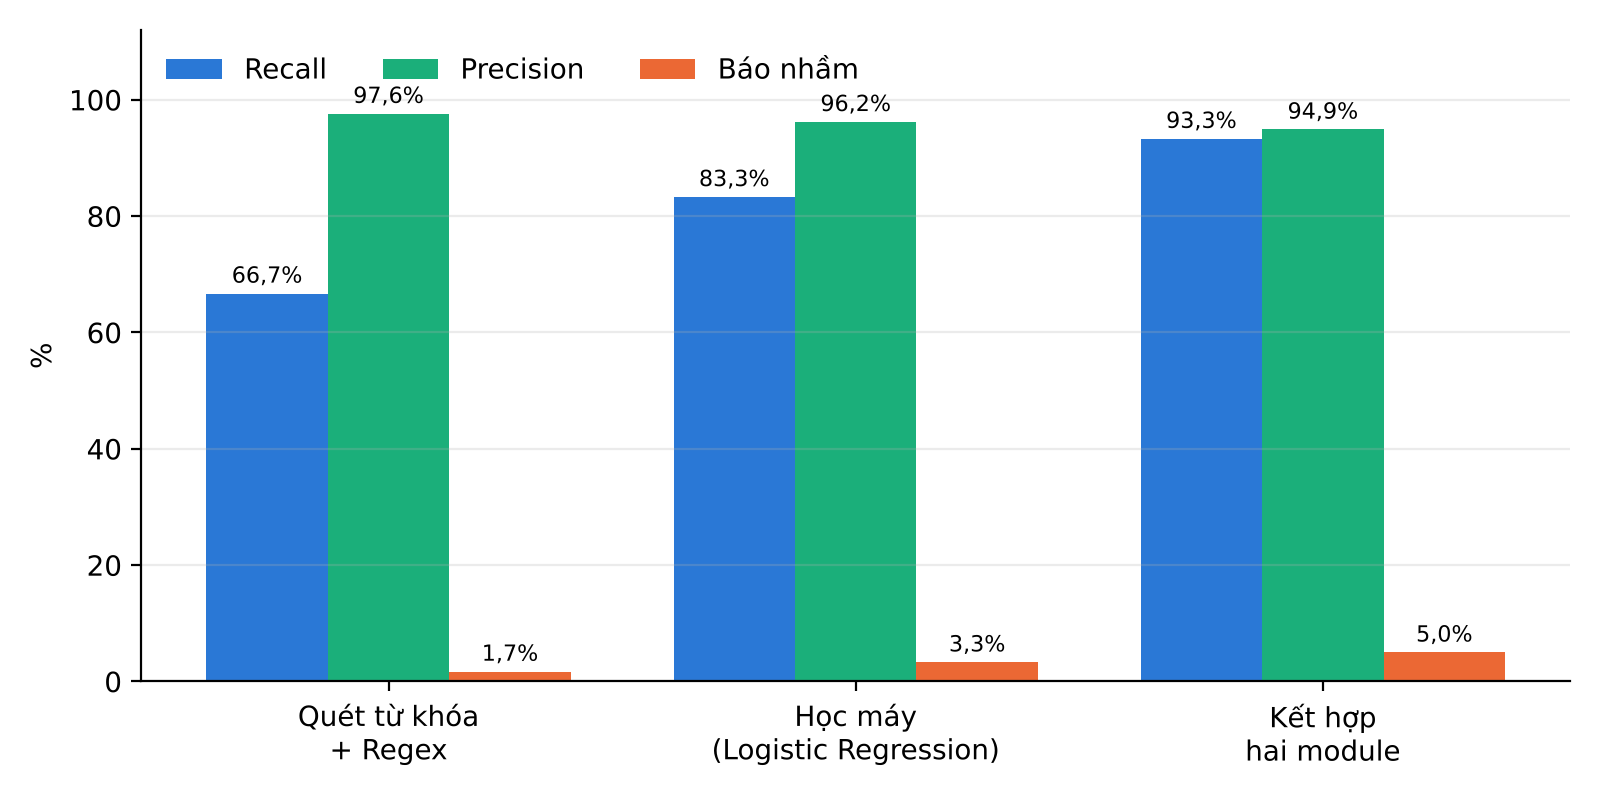
\includegraphics[width=0.85\textwidth]{figures/ket_qua_E1.png}
\caption{So sánh ba cách trên bộ kiểm tra 120 tin}
\label{fig:5.2}
\end{figure}

Về tốc độ, công cụ quét 46.000 tin mô phỏng trong khoảng 25 giây, tức gần 2.000 tin mỗi giây. Nếu một người đọc tay mất 30 giây cho mỗi tin, cùng khối lượng đó cần khoảng 383 giờ công, tương đương 48 ngày làm việc. Con số 46.000 lấy theo cỡ số gian hàng cơ quan điều tra công bố, nhưng đây là tin mô phỏng, không đại diện cho các gian hàng thật.

\paragraph{Demo trực tiếp}

Ô thử trực tiếp trong notebook cho phép nhập một tin bất kỳ và xem quyết định ngay. Ba tin dùng khi thuyết trình:

{\small\setstretch{1.1}
\begin{table}[H]
\centering
\caption{Kết quả demo trực tiếp}\label{tab:5.10}
\begin{tabularx}{\textwidth}{>{\hsize=1.099\hsize\raggedright\arraybackslash}X>{\hsize=0.548\hsize\raggedright\arraybackslash}X>{\hsize=1.353\hsize\raggedright\arraybackslash}X}
\toprule
\textbf{Tin nhập} & \textbf{Quyết định} & \textbf{Lý do công cụ đưa ra} \\
\midrule
Pass d.a.t.a khách mua bảo hiểm 5k số, mẫu 0912345678, 0987654321 & CHẶN (mua bán dữ liệu, điểm 0,95) & Từ khóa “data”, “data khách”; có mẫu dữ liệu cá nhân gồm 2 số điện thoại \\
Cho thuê sim nhận 0tp theo lượt, giao mã trong 30 giây. LH 0912345678 & CHẶN (dịch vụ xác thực hộ, điểm 0,81) & Từ khóa “otp”, “sim nhận”, “thuê sim”; “0tp” đã được chuẩn hóa thành “otp” \\
Khóa học nhận diện tin nhắn OTP giả mạo, phòng tránh lừa đảo. LH 0901222333 & CHO PHÉP (điểm 0,27) & Có từ “OTP” nhưng bị trừ điểm vì ngữ cảnh hợp lệ (“khóa học”); một số điện thoại liên hệ không bị tính là dữ liệu cá nhân \\
\bottomrule
\end{tabularx}
\end{table}}

\begin{figure}[H]
\centering
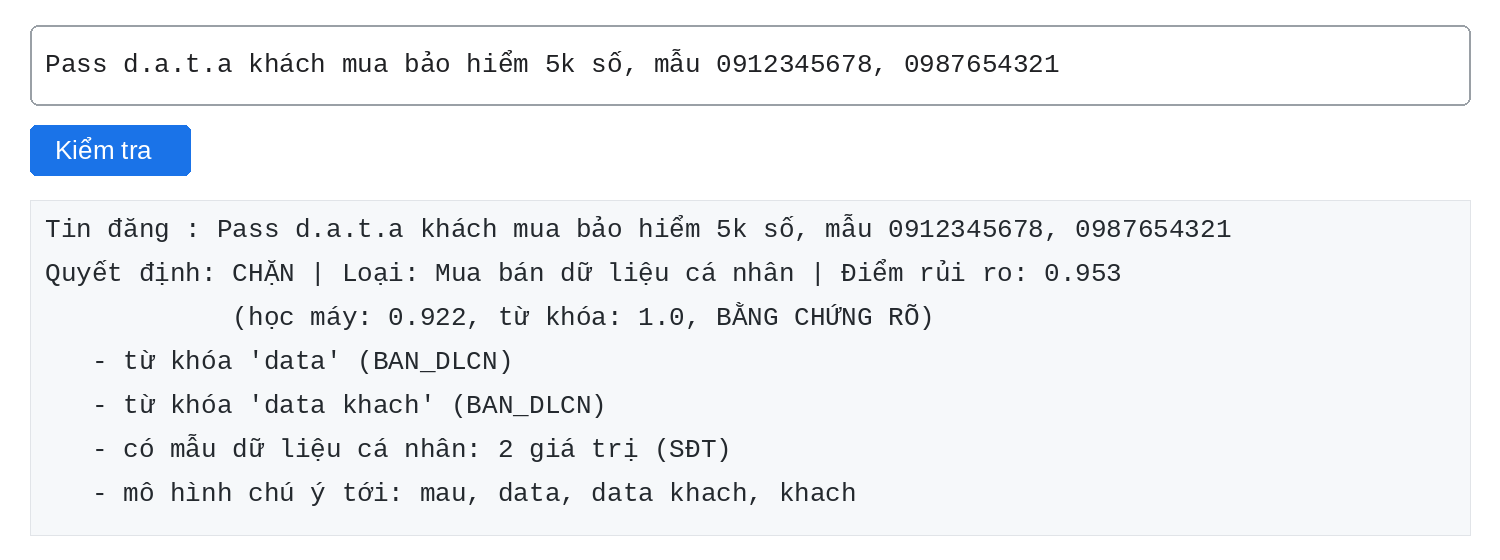
\includegraphics[width=0.95\textwidth]{figures/demo_truc_tiep.png}
\caption{Ô thử trực tiếp trong notebook với tin thứ nhất}
\label{fig:5.3}
\end{figure}

Mỗi tin bị gắn cờ được ghi vào nhật ký bằng chứng gồm thời điểm, quyết định, loại vi phạm, điểm rủi ro, lý do, nội dung đã che dữ liệu cá nhân (ví dụ “091*****78”) và mã băm SHA-256 của nội dung gốc để chứng minh nội dung không bị sửa sau khi ghi nhận. Nhật ký xuất ra file CSV và là đầu vào cho quy trình xử lý ở~\ref{sec:5.2.2}.

\paragraph{Tuân thủ khi triển khai thực tế}

Demo chỉ dùng dữ liệu tự tạo nên không xử lý dữ liệu cá nhân thật. Khi chạy trên tin đăng thật, công cụ vừa xử lý dữ liệu cá nhân của người bán và của những người có dữ liệu bị rao bán, vừa là một hệ thống trí tuệ nhân tạo. Vì vậy công cụ phải đáp ứng Luật Bảo vệ dữ liệu cá nhân 2025~\cite{luat-bvdlcn-2025}, Nghị định 356/2025/NĐ-CP~\cite{nd356-2025}, Luật Trí tuệ nhân tạo 2025~\cite{luat-ai-2025} và Nghị định 142/2026/NĐ-CP~\cite{nd142-2026}. Bảng dưới đây nêu từng yêu cầu và cách công cụ đáp ứng.

{\small\setstretch{1.1}
\begin{xltabular}{\textwidth}{>{\hsize=0.62\hsize\raggedright\arraybackslash}X>{\hsize=0.78\hsize\raggedright\arraybackslash}X>{\hsize=1.6\hsize\raggedright\arraybackslash}X}
\caption{Yêu cầu pháp lý khi triển khai công cụ phát hiện tin đăng}\label{tab:5.tuanthu}\\
\toprule
\textbf{Yêu cầu} & \textbf{Căn cứ} & \textbf{Cách đáp ứng} \\
\midrule
\endfirsthead
\toprule
\textbf{Yêu cầu} & \textbf{Căn cứ} & \textbf{Cách đáp ứng} \\
\midrule
\endhead
\bottomrule
\endlastfoot
Có căn cứ và đúng mục đích xử lý & Luật BVDLCN 2025: khoản 1 Điều 19, khoản 1 Điều 30; Nghị định 356/2025: Điều 19 & Chỉ quét tin đăng để phát hiện vi phạm, theo yêu cầu hoặc phối hợp với cơ quan có thẩm quyền; không dùng dữ liệu quét được cho mục đích khác. Lập hồ sơ đánh giá tác động xử lý dữ liệu cá nhân trước khi vận hành. \\
Dữ liệu huấn luyện hợp pháp & Luật Trí tuệ nhân tạo 2025: khoản 3 Điều 7 & Huấn luyện bằng dữ liệu tự tạo hoặc tin đăng đã khử nhận dạng; không dùng dữ liệu rò rỉ làm dữ liệu huấn luyện. \\
Mô hình không lưu dữ liệu cá nhân & Luật BVDLCN 2025: khoản 3 Điều 30 & Thay mọi dãy chữ số bằng một ký hiệu chung trước khi huấn luyện, để từ vựng của mô hình không chứa mảnh số điện thoại hay số CCCD. Mã hóa và phân quyền truy cập file mô hình. \\
Bảo vệ kết quả suy luận & Nghị định 356/2025: khoản 2 Điều 10 & Kết luận “gian hàng X có dấu hiệu bán dữ liệu” gắn với một người cụ thể nên cũng là dữ liệu cá nhân. Nhật ký bằng chứng chỉ lưu nội dung đã che và mã băm, chỉ người duyệt được xem, và có thời hạn lưu. \\
Con người quyết định cuối cùng & Luật Trí tuệ nhân tạo 2025: khoản 2 Điều 4, khoản 4 Điều 7 & CHẶN chỉ tạm ẩn tin và chuyển người duyệt xác nhận. Công cụ không tự gỡ tin hay khóa tài khoản. \\
Minh bạch và khiếu nại & Nghị định 356/2025: khoản 3 Điều 10; Luật Trí tuệ nhân tạo 2025: Điều 14 & Thông báo cho người bán rằng tin đăng được quét tự động, gửi kèm lý do bị gắn cờ (danh sách lý do do công cụ xuất ra) và kênh khiếu nại. \\
Phân loại rủi ro trước khi dùng & Luật BVDLCN 2025: khoản 4 Điều 30; Luật Trí tuệ nhân tạo 2025: Điều 9; Nghị định 142/2026: Điều 5 & Công cụ không tạo nội dung, không tương tác trực tiếp với công chúng, và người duyệt ra quyết định cuối, nên có cơ sở xếp vào mức rủi ro thấp. Trước khi dùng vẫn phải đối chiếu với Danh mục hệ thống trí tuệ nhân tạo rủi ro cao. \\
\end{xltabular}}

Nhóm đã thử bước thay chữ số trên notebook. Sau khi thay, từ vựng của mô hình không còn đặc trưng nào chứa từ ba chữ số liền nhau trở lên. Recall của riêng module học máy giảm từ 83,3\% xuống 80,0\%, còn kết quả của cách kết hợp hai module không đổi (recall 93,3\%, báo nhầm 5,0\%), vì số điện thoại và số CCCD vẫn do biểu thức chính quy nhận diện.

Quyền không tham gia xử lý tự động theo khoản 3 Điều 10 Nghị định 356/2025 khó áp dụng cho việc kiểm duyệt tin đăng bắt buộc trên sàn. Pháp luật hiện chưa quy định rõ trường hợp này.

\subsubsection{PoC tài liệu cho giải pháp 4 và 6: Bộ 3P xử lý sàn “chợ dữ liệu”}\label{sec:5.2.2}

PoC này cụ thể hóa giải pháp 4 và 6 theo cách tiếp cận 3P (Policy -- Process -- Procedure). Theo bài giảng về tuân thủ của môn học~\cite{lpsc-l6}, hệ thống quản lý an ninh thông tin của một tổ chức gồm chính sách, quy trình và thủ tục, và ba tầng này phải đối ứng với luật, quy định, hợp đồng bên ngoài. Ví dụ phân biệt: chính sách nêu điều phải đạt (“thông tin công ty trên máy tính phải được trả lại”), còn thủ tục nêu cách làm cụ thể (“phỏng vấn khi nghỉ việc và cách thu hồi tài liệu nhạy cảm”). PoC dùng ba tầng như sau:

{\small\setstretch{1.1}
\begin{table}[H]
\centering
\caption{Ba tầng 3P của PoC}\label{tab:5.3p}
\begin{tabularx}{\textwidth}{>{\raggedright\arraybackslash}l>{\hsize=0.8\hsize\raggedright\arraybackslash}X>{\hsize=1.2\hsize\raggedright\arraybackslash}X}
\toprule
\textbf{Tầng} & \textbf{Trả lời câu hỏi} & \textbf{Tài liệu trong PoC} \\
\midrule
Chính sách (Policy) & Phải đạt điều gì, theo căn cứ nào & Sáu cam kết: Đăng ký, Hàng cấm, Gỡ tin, Lưu trữ, Phối hợp theo vòng đời tin đăng; Giáo dục xuyên suốt (bảng~\ref{tab:5.cs}, \ref{tab:5.csdk}) \\
Quy trình (Process) & Gồm những bước nào, theo thứ tự nào & Luồng A, luồng B của nền tảng; phía cơ quan: bộ tiêu chí (bảng~\ref{tab:5.11}) và năm bước xử lý (hình~\ref{fig:5.4}) \\
Thủ tục (Procedure) & Ở mỗi bước: ai làm, làm gì, trong bao lâu & Thủ tục luồng A, B kèm ví dụ áp vào taphoammo (bảng~\ref{tab:5.tt}, \ref{tab:5.ttb}) và biểu mẫu tố giác (bảng~\ref{tab:5.12}) \\
\bottomrule
\end{tabularx}
\end{table}}

PoC nhắm vào ba thách thức ở chương 4 mà giải pháp 4 (Kiểm soát người bán) và giải pháp 6 (Phối hợp xử lý) phụ trách: Hạ tầng ở nước ngoài, Vỏ bọc doanh nghiệp và Dữ liệu nằm ở nhiều bên. Căn cứ là khung pháp luật hiện hành như đã nêu ở mục~\ref{sec:2.2.3}: Luật An ninh mạng 2025~\cite{luat-anm-2025}, Luật Bảo vệ dữ liệu cá nhân 2025~\cite{luat-bvdlcn-2025}, Nghị định 327/2026/NĐ-CP~\cite{nd327-2026} và Nghị định 333/2026/NĐ-CP~\cite{nd333-2026} (hai nghị định có hiệu lực từ 19/8/2026). PoC không áp ngược các văn bản này cho hành vi của taphoammo.net trước đó. Cảnh báo và nhật ký bằng chứng từ công cụ ở~\ref{sec:5.2.1} là một nguồn đầu vào của quy trình.

\paragraph{Tầng 1 -- Chính sách}

Sáu cam kết dưới đây là chính sách mà một nền tảng có gian hàng (sàn thương mại điện tử, chợ tài nguyên số) phải công bố và tuân thủ. Mỗi cam kết lấy nguyên ý từ một nghĩa vụ hoặc điều cấm trong luật. Thay vì đánh số, mỗi chính sách được gọi bằng một từ khóa và xếp theo vòng đời của một tin đăng trên sàn: đăng ký tài khoản, đăng tin, lưu trữ dữ liệu, và khi cơ quan chức năng có yêu cầu. Chính sách Giáo dục không gắn với một giai đoạn mà áp dụng xuyên suốt cho người vận hành các bước đó; chính sách này xuất phát từ nghĩa vụ tuyên truyền, phổ biến pháp luật của nhà cung cấp dịch vụ (điểm g khoản 2 Điều 6 Nghị định 327/2026).

{\small\setstretch{1.1}
\begin{table}[H]
\centering
\caption{Chính sách của nền tảng theo vòng đời một tin đăng}\label{tab:5.cs}
\begin{tabularx}{\textwidth}{>{\raggedright\arraybackslash}l>{\hsize=1.2\hsize\raggedright\arraybackslash}X>{\raggedright\arraybackslash}l>{\hsize=1.1\hsize\raggedright\arraybackslash}X>{\hsize=0.7\hsize\raggedright\arraybackslash}X}
\toprule
\textbf{Chính sách} & \textbf{Nội dung cam kết} & \textbf{Ai} & \textbf{Căn cứ} & \textbf{Thách thức} \\
\midrule
\multicolumn{5}{l}{\textit{Giai đoạn đăng ký}} \\
\textbf{Đăng ký} & Xác thực thông tin khi đăng ký tài khoản; chỉ tài khoản đã xác thực mới được đăng tin & Nền tảng & Luật ANM 2025: điểm a khoản 2 Điều 25; NĐ 333/2026: điểm a, d khoản 2 Điều 16 & Dữ liệu nằm ở nhiều bên (xác định người đứng sau gian hàng) \\
\multicolumn{5}{l}{\textit{Giai đoạn đăng tin}} \\
\textbf{Hàng cấm} & Không đăng bán dữ liệu cá nhân, tài khoản số, dịch vụ xác thực tài khoản hộ & Người dùng & Luật BVDLCN 2025: khoản 6 Điều 7; Luật ANM 2025: điểm h khoản 2 Điều 7, điểm g khoản 4 Điều 13 & Vỏ bọc doanh nghiệp (danh tính hợp lệ không làm hàng hóa hợp lệ) \\
\textbf{Gỡ tin} & Chủ động phát hiện, ngăn chặn và kịp thời gỡ bỏ tin xâm phạm bí mật cá nhân, đời sống riêng tư & Nền tảng & Luật ANM 2025: điểm b khoản 2 Điều 15 & Vỏ bọc doanh nghiệp \\
\multicolumn{5}{l}{\textit{Giai đoạn lưu trữ}} \\
\textbf{Lưu trữ} & Lưu dữ liệu người dùng tại Việt Nam (tối thiểu 24 tháng); nhật ký hệ thống truy xuất được ít nhất 12 tháng & Nền tảng & Luật ANM 2025: khoản 3 Điều 25; NĐ 333/2026: khoản 1, 2 Điều 19, khoản 1 Điều 20, điểm c khoản 6 Điều 16 & Hạ tầng ở nước ngoài \\
\multicolumn{5}{l}{\textit{Khi cơ quan chức năng có yêu cầu}} \\
\textbf{Phối hợp} & Chỉ định đầu mối phối hợp, tiếp nhận yêu cầu khẩn cấp theo chế độ thường trực 24/24 giờ; cung cấp thông tin, gỡ bỏ trong thời hạn luật định & Nền tảng & NĐ 327/2026: khoản 2 Điều 14; Luật ANM 2025: điểm a, b khoản 2 Điều 25 & Dữ liệu nằm ở nhiều bên \\
\multicolumn{5}{l}{\textit{Xuyên suốt các giai đoạn}} \\
\textbf{Giáo dục} & Phổ biến pháp luật và các thủ đoạn vi phạm mới cho người duyệt, đầu mối phối hợp, người vận hành hệ thống & Nền tảng & NĐ 327/2026: điểm g, điểm a khoản 2 Điều 6; NĐ 329/2026: khoản 1, điểm đ khoản 4 Điều 6~\cite{nd329-2026} & Vỏ bọc doanh nghiệp \\
\bottomrule
\end{tabularx}
\end{table}}

\paragraph{Vì sao là sáu chính sách này: PoC giải quyết gì, không giải quyết gì}

Chín thách thức ở chương 4 không cùng một loại, nên không cùng một cách giải. Bảng~\ref{tab:5.pv} xếp chúng theo cách giải, dựa trên bảng~\ref{tab:5.6}. PoC tài liệu chỉ nhận ba thách thức mà lời giải là quy định ai làm gì, trong bao lâu; đó đúng là nội dung của chính sách, quy trình và thủ tục.

{\small\setstretch{1.1}
\begin{table}[H]
\centering
\caption{Thách thức nào PoC tài liệu giải quyết}\label{tab:5.pv}
\begin{tabularx}{\textwidth}{>{\hsize=1.1\hsize\raggedright\arraybackslash}X>{\hsize=1.0\hsize\raggedright\arraybackslash}X>{\hsize=0.9\hsize\raggedright\arraybackslash}X}
\toprule
\textbf{Thách thức (chương 4)} & \textbf{Giải bằng} & \textbf{Giải pháp (mục~\ref{sec:5.1})} \\
\midrule
Hạ tầng ở nước ngoài; Vỏ bọc doanh nghiệp; Dữ liệu nằm ở nhiều bên & \textbf{Quy định ai làm gì, trong bao lâu: PoC tài liệu 3P} & 4 -- Kiểm soát người bán; 6 -- Phối hợp xử lý \\
Khối lượng lớn; Cách viết lách bộ lọc & Công cụ phát hiện & 1 -- Phát hiện tin có dấu hiệu vi phạm (demo) \\
Nhiều văn bản, hiệu lực khác nhau theo thời gian; Ranh giới trách nhiệm giữa người bán và sàn & Phân tích pháp lý & 5 -- Ma trận trách nhiệm pháp lý (đề xuất) \\
Tài khoản đổi chủ; Dữ liệu dễ sao chép & Bên khác, không phải sàn: nền tảng gốc của tài khoản, bên kiểm soát dữ liệu & 2 -- Bảo vệ tài khoản trên nền tảng gốc; 3 -- Truy nguồn rò rỉ dữ liệu (đề xuất) \\
\bottomrule
\end{tabularx}
\end{table}}

Với ba thách thức PoC nhận, bảng~\ref{tab:5.csdk} đi từ dữ kiện đã công bố ở chương 3 tới chính sách tương ứng. Cụm từ in đậm trong cột dữ kiện là chỗ thể hiện thách thức.

{\small\setstretch{1.1}
\begin{table}[H]
\centering
\caption{Thách thức, dữ kiện vụ việc và chính sách tương ứng}\label{tab:5.csdk}
\begin{tabularx}{\textwidth}{>{\hsize=0.7\hsize\raggedright\arraybackslash}X>{\hsize=1.3\hsize\raggedright\arraybackslash}X>{\hsize=1.1\hsize\raggedright\arraybackslash}X>{\hsize=0.9\hsize\raggedright\arraybackslash}X}
\toprule
\textbf{Thách thức} & \textbf{Dữ kiện} & \textbf{Chuyện gì đã xảy ra} & \textbf{Chính sách} \\
\midrule
Vỏ bọc doanh nghiệp & Công ty có đăng ký, \textbf{có kiểm duyệt người bán}, nhưng vẫn bán dữ liệu cá nhân, tài khoản, dịch vụ xác thực (mục~\ref{sec:3.1}, \ref{sec:3.2.1}) & Người bán được kiểm tra; hàng hóa không được kiểm tra, không bị gỡ & Hàng cấm, Gỡ tin, Giáo dục (riêng Đăng ký là chưa đủ) \\
Hạ tầng ở nước ngoài & Hơn 1,35 triệu tài khoản; \textbf{máy chủ ở nước ngoài}, tên miền đi thuê (mục~\ref{sec:3.2.2}) & Dữ liệu người dùng không có bản lưu trong nước; cơ quan điều tra nêu việc này gây khó truy vết & Lưu trữ \\
Dữ liệu nằm ở nhiều bên & Tin đăng, thanh toán, hạ tầng, quảng cáo nằm ở \textbf{sàn, ngân hàng hoặc ví điện tử, nhà cung cấp máy chủ, nền tảng quảng cáo} (mục~\ref{sec:3.2.3}, \ref{sec:3.2.4}, \ref{sec:4.3}) & Thông tin về người đứng sau gian hàng nằm rải rác ở nhiều bên, không có đầu mối, không có thời hạn & Đăng ký, Phối hợp \\
-- & Việc chạy quảng cáo (mục~\ref{sec:3.2.3}); làm trung gian thanh toán (mục~\ref{sec:3.2.4}) & -- & Ngoài phạm vi PoC; đối chiếu ở chương~\ref{sec:7} và pháp luật thanh toán \\
\bottomrule
\end{tabularx}
\end{table}}

\paragraph{Tầng 2 -- Quy trình: hai luồng của nền tảng}

Chính sách, quy trình và thủ tục là tài liệu của cùng một tổ chức. Quy trình của PoC vì vậy được viết cho nền tảng, gồm hai luồng:

\begin{itemize}
\item \textbf{Luồng A -- nền tảng tự kiểm soát:} Đăng ký $\rightarrow$ Duyệt tin $\rightarrow$ Gỡ tin $\rightarrow$ Lưu trữ. Luồng này thực hiện các chính sách Đăng ký, Hàng cấm, Gỡ tin và Lưu trữ. Cảnh báo từ công cụ ở~\ref{sec:5.2.1} là đầu vào của bước Duyệt tin. Chính sách Giáo dục áp dụng xuyên suốt cả hai luồng cho người thực hiện các bước.
\item \textbf{Luồng B -- nền tảng phối hợp với cơ quan:} Nhận yêu cầu $\rightarrow$ Xác thực $\rightarrow$ Thực hiện $\rightarrow$ Phản hồi. Luồng này thực hiện chính sách Phối hợp. Khoản 2 Điều 14 Nghị định 327/2026 áp dụng cho chủ quản hệ thống thông tin, nhà cung cấp dịch vụ và cơ quan, tổ chức có liên quan~\cite{nd327-2026}, nên cùng luồng này áp dụng cho các bên khác đang giữ dữ liệu của vụ việc như ngân hàng hoặc ví điện tử, nhà cung cấp máy chủ, nền tảng quảng cáo (thách thức Dữ liệu nằm ở nhiều bên).
\end{itemize}

\paragraph{Tầng 2 -- Quy trình phía cơ quan chức năng: bộ tiêu chí nhận diện “chợ dữ liệu”}

Khi chính nhà vận hành cố ý vi phạm như taphoammo.net, nền tảng sẽ không tự áp dụng luồng A. Phần việc lúc này thuộc cơ quan chức năng: nhận diện sàn, chuyển đúng thẩm quyền và gửi yêu cầu vào luồng B của sàn và của các bên giữ dữ liệu. Bộ tiêu chí giúp người kiểm tra quyết định một sàn có cần được xem xét như một “chợ dữ liệu” hay không. Mỗi tiêu chí xây từ một đặc điểm đã công bố của taphoammo~\cite{bca-2026}.

{\small\setstretch{1.1}
\begin{table}[H]
\centering
\caption{Bộ tiêu chí nhận diện “chợ dữ liệu”, căn cứ theo luật hiện hành}\label{tab:5.11}
\begin{tabularx}{\textwidth}{>{\raggedright\arraybackslash}l>{\hsize=0.6\hsize\raggedright\arraybackslash}X>{\hsize=1.15\hsize\raggedright\arraybackslash}X>{\hsize=1.25\hsize\raggedright\arraybackslash}X>{\hsize=1.0\hsize\raggedright\arraybackslash}X}
\toprule
\textbf{STT} & \textbf{Tiêu chí} & \textbf{Dấu hiệu kiểm tra} & \textbf{Căn cứ} & \textbf{Đặc điểm tương ứng ở taphoammo} \\
\midrule
1 & Hàng hóa đăng bán & Đăng bán dữ liệu cá nhân, thông tin tài khoản số, dịch vụ xác thực tài khoản hộ; có thể dùng công cụ ở~\ref{sec:5.2.1} để sàng lọc & Luật BVDLCN 2025: khoản 6 Điều 7; Luật ANM 2025: điểm g khoản 4 Điều 13; NĐ 330/2026: điểm c khoản 2 Điều 14 & Đăng bán công khai dữ liệu cá nhân, tài khoản mạng xã hội và thư điện tử \\
2 & Thu phí trung gian & Sàn nhận, giữ, chuyển tiền thay người mua, người bán và thu phí trên mỗi giao dịch & NĐ 330/2026: điểm b khoản 2 Điều 14; NĐ 340/2025: khoản 6 Điều 31 & Thu phí 3--5\% mỗi giao dịch \\
3 & Kiểm duyệt người bán & Sàn có duyệt gian hàng nhưng vẫn để hàng hóa vi phạm tồn tại & NĐ 327/2026: khoản 10 Điều 10; NĐ 330/2026: điểm e khoản 2 Điều 15 & Có kiểm duyệt người bán \\
4 & Quảng cáo đa nền tảng & Sàn được quảng cáo trên mạng xã hội, công cụ tìm kiếm & NĐ 330/2026: điểm d khoản 3 Điều 14; NĐ 327/2026: điểm a khoản 2 Điều 6 (nền tảng quảng cáo phải rà soát) & Quảng cáo trên Facebook, Telegram, TikTok, Instagram, Google \\
5 & Hạ tầng ở nước ngoài & Doanh nghiệp trong nước đặt máy chủ ở nước ngoài, không có bản lưu dữ liệu người dùng trong nước & Luật ANM 2025: khoản 3 Điều 25; NĐ 333/2026: khoản 2 Điều 19; NĐ 330/2026: điểm c khoản 2 Điều 29, điểm a khoản 1 Điều 33 & Máy chủ ở nước ngoài, thuê tên miền \\
6 & Vỏ bọc doanh nghiệp & Có đăng ký doanh nghiệp nhưng ngành nghề không khớp hàng hóa thực tế & NĐ 330/2026: điểm đ khoản 1 Điều 53; NĐ 327/2026: khoản 10 Điều 10 & Đứng tên Công ty TNHH Phát triển Công nghệ số HCT \\
\bottomrule
\end{tabularx}
\end{table}}

Mỗi tiêu chí dựa trên một điều cấm, nghĩa vụ hoặc hành vi bị xử phạt trong khung pháp luật hiện hành~\cite{luat-anm-2025,luat-bvdlcn-2025,nd327-2026,nd330-2026,nd333-2026,nd340-2025}. Cách đánh giá là quy tắc do nhóm đề xuất cho PoC: tiêu chí 1 (hàng hóa đăng bán) là điều kiện bắt buộc. Sàn thỏa tiêu chí 1 và ít nhất hai tiêu chí khác thì được chuyển sang quy trình xử lý; sàn chỉ thỏa tiêu chí 1 được đưa vào danh sách theo dõi. Áp vào taphoammo.net, cột cuối của bảng~\ref{tab:5.11} cho thấy sàn thỏa cả sáu tiêu chí bằng dữ kiện đã công bố.

\paragraph{Tầng 2 -- Quy trình phía cơ quan chức năng: năm bước xử lý khi một sàn bị nhận diện}

Quy trình nối tiếp kết quả của công cụ ở~\ref{sec:5.2.1} và cụ thể hóa giải pháp 6 ở~\ref{sec:5.1}. Bộ tiêu chí ở trên được dùng tại bước sàng lọc. Bảng~\ref{tab:5.ttcq} ghi căn cứ của từng bước và sự kiện tương ứng trong vụ việc. Các mốc vụ việc diễn ra trước khi Luật An ninh mạng 2025 và các nghị định hướng dẫn có hiệu lực; cột cuối chỉ cho biết sự kiện thật ứng với từng bước, không có nghĩa các điều khoản này đã được áp dụng.

{\small\setstretch{1.1}
\begin{xltabular}{\textwidth}{>{\raggedright\arraybackslash}l>{\hsize=1.2\hsize\raggedright\arraybackslash}X>{\hsize=0.95\hsize\raggedright\arraybackslash}X>{\hsize=0.85\hsize\raggedright\arraybackslash}X}
\caption{Quy trình phía cơ quan chức năng: căn cứ và đối chiếu vụ việc}\label{tab:5.ttcq}\\
\toprule
\textbf{Bước} & \textbf{Cơ quan làm gì} & \textbf{Căn cứ} & \textbf{Trong vụ việc} \\
\midrule
\endfirsthead
\toprule
\textbf{Bước} & \textbf{Cơ quan làm gì} & \textbf{Căn cứ} & \textbf{Trong vụ việc} \\
\midrule
\endhead
\bottomrule
\endlastfoot
1. Tiếp nhận & Nhận cảnh báo (kể cả từ công cụ ở~\ref{sec:5.2.1}), tố giác của tổ chức, cá nhân và nhà cung cấp dịch vụ, theo biểu mẫu ở bảng~\ref{tab:5.12} & NĐ 327/2026: khoản 5 Điều 10, khoản 1 Điều 11, khoản 1 Điều 14; NĐ 329/2026: điểm d khoản 2 Điều 5 & 6/2025: lập chuyên án sau khi phát hiện qua nắm tình hình trên không gian mạng \\
2. Sàng lọc, xác minh & Chấm sáu tiêu chí; xác minh tài khoản số, địa chỉ mạng, đường dẫn & NĐ 327/2026: khoản 2 Điều 9, khoản 3 Điều 11 & Thỏa 6/6 tiêu chí (bảng~\ref{tab:5.11}) \\
3. Thu thập dữ liệu điện tử & Dữ liệu điện tử không bị can thiệp, thay đổi; quá trình thu thập được ghi biên bản, hình ảnh và có thể lặp lại; che dữ liệu cá nhân khi lưu hồ sơ & NĐ 333/2026: khoản 3 Điều 12 & 2/2026: khám xét, thu giữ máy tính và dữ liệu điện tử \\
4. Áp dụng biện pháp & Yêu cầu cung cấp thông tin, xóa bỏ thông tin (luồng B của sàn và các bên giữ dữ liệu) và kiểm tra việc chấp hành; yêu cầu phong tỏa tài khoản số, tạm dừng giao dịch; đình chỉ hệ thống thông tin, đề nghị Bộ Khoa học và Công nghệ thu hồi tên miền (trường hợp cấp bách: yêu cầu trực tiếp, văn bản chậm nhất 24 giờ sau đó); doanh nghiệp Việt Nam phối hợp ngăn chặn dịch vụ qua biên giới vi phạm & NĐ 327/2026: khoản 3, 4 Điều 9; NĐ 333/2026: khoản 2 Điều 11, khoản 2, 4 Điều 13, khoản 3 Điều 14 & Áp vào: yêu cầu ngân hàng, ví điện tử phong tỏa tài khoản nhận tiền của sàn; đề nghị thu hồi tên miền taphoammo.net \\
5. Chuyển thẩm quyền, xử lý & Bộ Công an là đầu mối chủ trì với hoạt động dân sự, kinh tế; hành vi thuộc chuyên ngành khác (ví dụ trung gian thanh toán) áp dụng nghị định chuyên ngành; có dấu hiệu tội phạm thì chuyển hồ sơ truy cứu trách nhiệm hình sự & NĐ 333/2026: điểm a khoản 5 Điều 14; NĐ 329/2026: điểm a khoản 3 Điều 9; NĐ 330/2026: khoản 3 Điều 1, khoản 4 Điều 4; Luật ANM 2025: điểm n khoản 1 Điều 5 & 25/12/2025: khởi tố vụ án; 7/2026: công bố khởi tố 3 bị can về tội theo Điều 288 Bộ luật Hình sự \\
\end{xltabular}}

\begin{figure}[H]
\centering
% Quy trình xử lý khi một sàn bị nhận diện (bản sơ bộ, Người 5 có thể thay)
\setstretch{1}
\begin{tikzpicture}[font=\small, node distance=0.4cm,
  box/.style={draw, rounded corners=2pt, align=center, minimum height=1.3cm, text width=2.3cm, fill=blue!7},
  arr/.style={-{Stealth[length=2mm]}, thick}]
  \node[box] (a) {Tiếp nhận};
  \node[box, right=of a] (b) {Sàng lọc theo\\bộ tiêu chí};
  \node[box, right=of b] (c) {Bảo toàn\\chứng cứ};
  \node[box, right=of c] (d) {Chuyển đúng\\thẩm quyền};
  \node[box, right=of d] (e) {Theo dõi và\\phản hồi};
  \foreach \u/\v in {a/b, b/c, c/d, d/e} \draw[arr] (\u) -- (\v);
\end{tikzpicture}

\caption{Quy trình phía cơ quan chức năng khi một sàn bị nhận diện}
\label{fig:5.4}
\end{figure}

\paragraph{Tầng 3 -- Thủ tục cho từng bước}

Thủ tục ghi rõ ở mỗi bước ai làm, làm gì và trong thời hạn nào. Các thời hạn trong bảng đều lấy từ văn bản pháp luật; bước nào luật không quy định thời hạn thì ghi “không quy định”. Cột cuối áp thủ tục vào taphoammo.net bằng các dữ kiện đã công bố~\cite{bca-2026}, để thấy mỗi thủ tục trông ra sao trong một vụ việc cụ thể.

{\small\setstretch{1.1}
\begin{xltabular}{\textwidth}{>{\raggedright\arraybackslash}l>{\hsize=1.25\hsize\raggedright\arraybackslash}X>{\hsize=0.6\hsize\raggedright\arraybackslash}X>{\hsize=0.8\hsize\raggedright\arraybackslash}X>{\hsize=1.05\hsize\raggedright\arraybackslash}X}
\caption{Thủ tục luồng A -- nền tảng tự kiểm soát}\label{tab:5.tt}\\
\toprule
\textbf{Bước} & \textbf{Thủ tục (ai, làm gì)} & \textbf{Thời hạn} & \textbf{Căn cứ} & \textbf{Áp vào taphoammo} \\
\midrule
\endfirsthead
\toprule
\textbf{Bước} & \textbf{Thủ tục (ai, làm gì)} & \textbf{Thời hạn} & \textbf{Căn cứ} & \textbf{Áp vào taphoammo} \\
\midrule
\endhead
\bottomrule
\endlastfoot
Đăng ký & Nền tảng xác thực tài khoản bằng số điện thoại di động tại Việt Nam, hoặc bằng số định danh cá nhân; tài khoản chưa xác thực không được đăng tin & Khi đăng ký tài khoản & NĐ 333/2026: điểm a, b, d khoản 2 Điều 16 & Sàn đã có kiểm duyệt người bán; riêng bước này không ngăn được hàng cấm \\
Duyệt tin & Công cụ ở~\ref{sec:5.2.1} chấm mỗi tin mới (CHẶN, CHUYỂN NGƯỜI DUYỆT, CHO PHÉP); người duyệt quyết định với tin bị gắn cờ & Không quy định & Luật ANM 2025: điểm b khoản 2 Điều 15; Luật BVDLCN 2025: khoản 6 Điều 7 & Gian hàng bán tài khoản Facebook, TikTok, Telegram, Instagram, thư điện tử thuộc nhóm “mua bán tài khoản” mà công cụ gắn cờ \\
Gỡ tin & Ghi nhật ký xử lý tin, lưu bằng chứng (ảnh chụp, mã băm) rồi gỡ tin. Tài khoản đăng từ 03 tin vi phạm trở lên trong 30 ngày bị hạn chế hiển thị hoặc khóa tạm thời tối đa 60 ngày; từ 10 tin trở lên trong 90 ngày thì tối đa 180 ngày & “Kịp thời” & Luật ANM 2025: điểm b khoản 2 Điều 15; NĐ 333/2026: điểm d khoản 4, điểm b khoản 6 Điều 16 & Sàn có hơn 46.000 gian hàng; gian hàng đăng lặp lại tin vi phạm bị khóa theo các ngưỡng này \\
Lưu trữ & Lưu tại Việt Nam: thông tin cá nhân, tên tài khoản, thời gian sử dụng, địa chỉ IP đăng nhập, đăng xuất gần nhất, số điện thoại gắn với tài khoản. Nhật ký gồm tài khoản, thời gian đăng nhập, đăng xuất, địa chỉ IP, cổng nguồn và nhật ký xử lý tin đăng & Dữ liệu tối thiểu 24 tháng; nhật ký ít nhất 12 tháng & NĐ 333/2026: khoản 1, 2 Điều 19, khoản 1 Điều 20, điểm b, c khoản 6 Điều 16 & Hơn 1,35 triệu tài khoản trên máy chủ ở nước ngoài: phải có bản lưu các dữ liệu này trong nước \\
Giáo dục & Nền tảng (bộ phận thường trực bảo vệ an ninh mạng, nếu có) phổ biến pháp luật và các thủ đoạn vi phạm rà soát được cho người duyệt, đầu mối, người vận hành & Không quy định & NĐ 327/2026: điểm g, điểm a khoản 2 Điều 6; NĐ 329/2026: khoản 1, điểm đ khoản 4 Điều 6 & Nội dung lấy từ vụ việc: dữ liệu cá nhân, tài khoản mạng xã hội, thư điện tử, “dịch vụ xác thực tài khoản”; người bán đã xác thực không làm hàng hóa hợp pháp \\
\end{xltabular}}

{\small\setstretch{1.1}
\begin{xltabular}{\textwidth}{>{\raggedright\arraybackslash}l>{\hsize=1.2\hsize\raggedright\arraybackslash}X>{\hsize=0.65\hsize\raggedright\arraybackslash}X>{\hsize=0.8\hsize\raggedright\arraybackslash}X>{\hsize=1.05\hsize\raggedright\arraybackslash}X}
\caption{Thủ tục luồng B -- nền tảng phối hợp với cơ quan}\label{tab:5.ttb}\\
\toprule
\textbf{Bước} & \textbf{Thủ tục (ai, làm gì)} & \textbf{Thời hạn} & \textbf{Căn cứ} & \textbf{Áp vào taphoammo} \\
\midrule
\endfirsthead
\toprule
\textbf{Bước} & \textbf{Thủ tục (ai, làm gì)} & \textbf{Thời hạn} & \textbf{Căn cứ} & \textbf{Áp vào taphoammo} \\
\midrule
\endhead
\bottomrule
\endlastfoot
Nhận yêu cầu & Đầu mối phối hợp của nền tảng nhận yêu cầu bằng văn bản giấy, văn bản điện tử, đường dây nóng; yêu cầu khẩn cấp theo chế độ thường trực & 24/24 giờ & NĐ 327/2026: khoản 1 Điều 12, khoản 2 Điều 14 & Yêu cầu của lực lượng chuyên trách về các gian hàng bán dữ liệu cá nhân đến đầu mối của sàn \\
Xác thực & Xác thực chủ thể yêu cầu; bảo mật thông tin được cung cấp & Không quy định & NĐ 333/2026: điểm b khoản 3 Điều 16 & Chỉ gửi dữ liệu người dùng khi xác nhận yêu cầu đúng là của lực lượng chuyên trách thuộc Bộ Công an \\
Thực hiện & Cung cấp thông tin người dùng; ngăn chặn chia sẻ, xóa thông tin, gỡ dịch vụ theo yêu cầu & Cung cấp chậm nhất 24 giờ (khẩn cấp 03 giờ); gỡ bỏ chậm nhất 24 giờ (khẩn cấp 06 giờ) & Luật ANM 2025: điểm a, b khoản 2 Điều 25; NĐ 333/2026: điểm c khoản 3, điểm b khoản 4 Điều 16 & Với mỗi chủ gian hàng: tên tài khoản, thời gian sử dụng dịch vụ, thông tin thanh toán, địa chỉ IP (danh mục ở điểm d khoản 2 Điều 25 Luật ANM 2025) \\
Phản hồi & Thực hiện và phản hồi kết quả xử lý & Theo thời hạn trong yêu cầu & NĐ 327/2026: khoản 2 Điều 14 & Báo lại tin nào đã gỡ, dữ liệu nào đã cung cấp, vào thời điểm nào \\
\end{xltabular}}

Luồng A cùng các chính sách Đăng ký, Hàng cấm, Gỡ tin xử lý thách thức Vỏ bọc doanh nghiệp: kiểm tra danh tính người bán và kiểm tra hàng hóa là hai bước riêng. Chính sách Lưu trữ và bước thu hồi tên miền phía cơ quan (Điều 13 Nghị định 333/2026) xử lý thách thức Hạ tầng ở nước ngoài: không với tới được máy chủ ở nước ngoài, nhưng dữ liệu người dùng Việt Nam có bản lưu trong nước và tên miền có thể bị tạm ngừng, thu hồi. Luồng B xử lý thách thức Dữ liệu nằm ở nhiều bên: mỗi bên giữ dữ liệu có một đầu mối, có phương thức phối hợp và có thời hạn.

\paragraph{Biểu mẫu tiếp nhận tố giác}

Biểu mẫu là phần thủ tục của bước tiếp nhận trong quy trình phía cơ quan chức năng, gồm các trường sau:

{\small\setstretch{1.1}
\begin{table}[H]
\centering
\caption{Các trường của biểu mẫu tiếp nhận tố giác}\label{tab:5.12}
\begin{tabularx}{\textwidth}{>{\hsize=0.541\hsize\raggedright\arraybackslash}X>{\hsize=1.459\hsize\raggedright\arraybackslash}X>{\raggedright\arraybackslash}l}
\toprule
\textbf{Trường} & \textbf{Nội dung} & \textbf{Bắt buộc} \\
\midrule
Người tố giác & Họ tên và cách liên hệ; cho phép tố giác ẩn danh & Không \\
Đối tượng bị tố giác & Địa chỉ sàn, gian hàng hoặc đường dẫn tin đăng & Có \\
Loại hành vi nghi ngờ & Chọn trong bảy hành vi ở Chương 3, kèm mô tả ngắn & Có \\
Thời điểm phát hiện & Ngày, giờ phát hiện & Có \\
Bằng chứng & Ảnh chụp màn hình, đường dẫn; không gửi kèm dữ liệu cá nhân bị rò rỉ & Có \\
Cam kết & Thông tin cung cấp là trung thực; không gửi dữ liệu cá nhân ngoài phạm vi cần thiết & Có \\
Phần cơ quan tiếp nhận ghi & Mã hồ sơ, người tiếp nhận, kết quả sàng lọc theo bộ tiêu chí, đơn vị được chuyển hồ sơ & Có \\
\bottomrule
\end{tabularx}
\end{table}}


\paragraph{Kiểm tra độ phủ theo McCumber Cube}

McCumber Cube~\cite{lpsc-l1} có ba trục vẽ từ một gốc chung: tính chất cần bảo vệ (Confidentiality, Integrity, Availability), trạng thái của thông tin (Storage, Processing, Transmission) và nhóm biện pháp (Policy, Education, Technology). Các biện pháp được áp dụng đồng thời, bổ trợ nhau, và phải cân nhắc đánh đổi. Nhóm dùng ba trục này để kiểm tra bộ 3P và công cụ ở~\ref{sec:5.2.1} có bỏ trống chiều nào không:

{\small\setstretch{1.1}
\begin{table}[H]
\centering
\caption{Đối chiếu PoC với ba trục của McCumber Cube}\label{tab:5.mc}
\begin{tabularx}{\textwidth}{>{\raggedright\arraybackslash}l>{\raggedright\arraybackslash}l>{\hsize=1.3\hsize\raggedright\arraybackslash}X>{\hsize=0.7\hsize\raggedright\arraybackslash}X}
\toprule
\textbf{Trục} & \textbf{Thành phần} & \textbf{Phần của PoC đáp ứng} & \textbf{Ghi chú} \\
\midrule
\multirow{3}{*}{CIA} & Confidentiality & Hàng cấm, Gỡ tin: chặn việc đăng bán dữ liệu cá nhân, tài khoản & \\
 & Integrity & Gỡ tin (nhật ký xử lý, mã băm); bước thu thập dữ liệu điện tử phía cơ quan: dữ liệu không bị thay đổi & \\
 & Availability & Lưu trữ, Phối hợp: dữ liệu lưu trong nước, cung cấp trong 24 giờ & Cho cơ quan có thẩm quyền \\
\midrule
\multirow{3}{*}{Trạng thái} & Storage & Lưu trữ: lưu tại Việt Nam, nhật ký 12 tháng & \\
 & Processing & Đăng ký, Duyệt tin, công cụ ở~\ref{sec:5.2.1}: xác thực, quét tin đăng & \\
 & Transmission & Luồng B: xác thực chủ thể yêu cầu, bảo mật thông tin được cung cấp & \\
\midrule
\multirow{3}{*}{Biện pháp} & Policy & Sáu chính sách ở bảng~\ref{tab:5.cs} & \\
 & Technology & Công cụ ở~\ref{sec:5.2.1}, mã băm, xác thực tài khoản & \\
 & Education & Chính sách Giáo dục: phổ biến pháp luật, thủ đoạn vi phạm cho người duyệt, đầu mối, người vận hành & NĐ 327/2026 điểm g khoản 2 Điều 6 \\
\bottomrule
\end{tabularx}
\end{table}}

Trục Education được đáp ứng bằng chính sách Giáo dục. Luật không quy định tần suất phổ biến, nên thủ tục ghi “không quy định”; nội dung lấy từ các thủ đoạn mà nền tảng rà soát được (điểm a khoản 2 Điều 6 Nghị định 327/2026).
